\section{System Implementation}
\label{sec:design}

\begin{figure*}[h!]
\centering
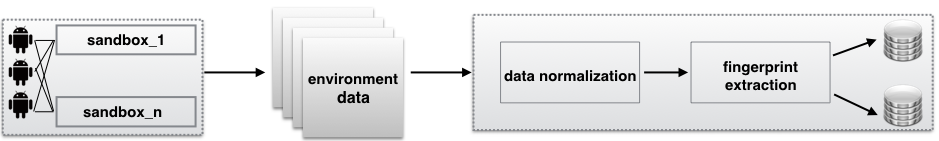
\includegraphics[keepaspectratio=true, width=1\textwidth]{system_design_001.png}
\caption{The design of fingerprint collector}
\label{fig:design}
\end{figure*}

\begin{figure}[h!]
\centering
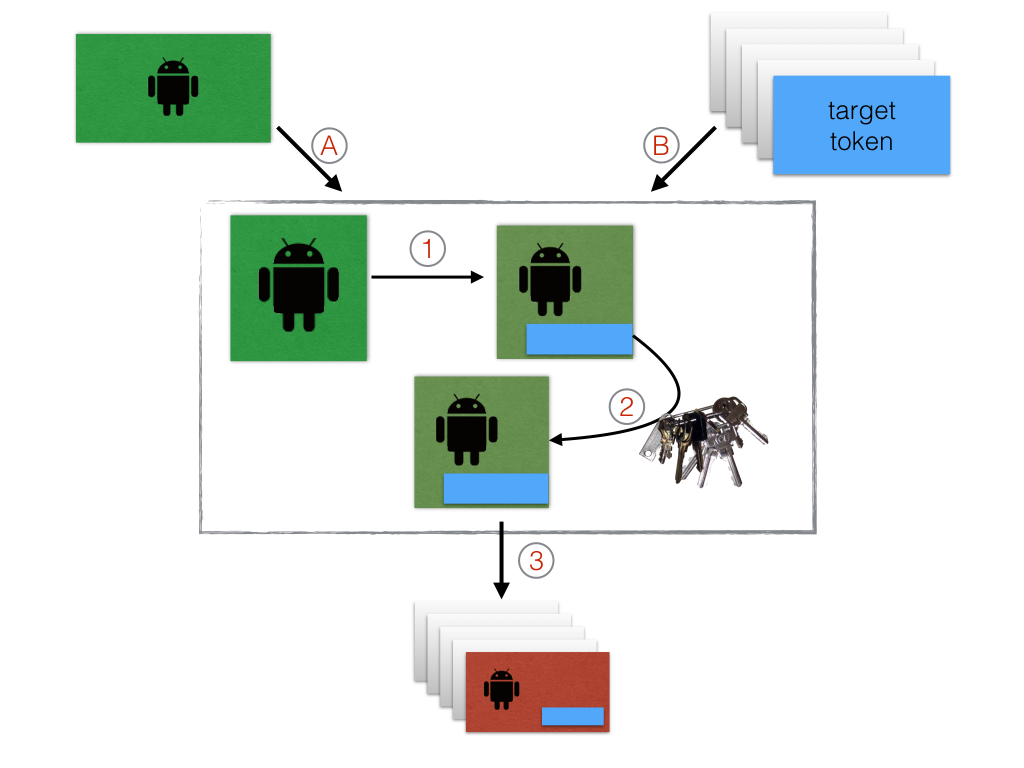
\includegraphics[keepaspectratio=true, width=\columnwidth]{scouter.png}
\caption{Scouting apps generator}
\label{fig:scouter}
\end{figure}

In this section, we present the design of the fingerprint collector. As depicted in Figure \ref{fig:design}, it consists of two components: (I) scouting-app and (II) fingerprint extractor. The scouting-app is used to collect usage-profile fingerprints. It uses only public Android APIs to get information about the execution environment. The app does not use native code, neither Java reflection nor code obfuscation techniques to hide its sensitive behaviors. The reason is that the prior static analysis in most analyzers would highly regard the scouting app as a benign app and filter it out if none suspicious evidence is found. To this end, and to make the fingerprint process even more stealthy as well we implemented several scouting-app each testing for a subset of usage-profile we were interested in. By following this approach we avoid to create a single application that requires a lot of sensitive privileges which could be marked as suspicious and then manually analyzed later on, instead we use several scouting-app such that none of those would require a suspicious combination of sensitive privileges.  \\
The scouting app uses different threads to execute the scouting logic. Each analysis sends its results back to the remote server in the JSON format. All types of collected fingerprints are shown in Table \ref{tab:data}. \\
% Differently from other works \cite{neuner2014enter}, where  sandbox detection uses by low level information like execution time
% All the collected data is strongly related to run-time environment \\

\begin{table}
\centering
\caption{ usage-profile Data }
\begin{tabular}{|c|c|} \hline
Type&Data\\ \hline
Contact & Name, numbers, email\\ \hline
Location & GPS, network, latitude, longitude \\ \hline
%Sensors & power, maxrange, resolution, vendor, version \\ \hline
SMS & inbox, send, draft\\ \hline
%System & fs, ps, uname, mount, df \\ \hline
WiFi & SSID, signal-strength  \\ \hline
App & package-name, version, hash \\ \hline
Battery & battery-level, stat, chargePlug \\ \hline
Call & recent calls \\
%Debugger & /proc/ , isDebuggerConnected \\ 
\hline
\end{tabular}
\label{tab:data}
\end{table}

To track which sandbox analyzes the scouting app, we need to build a scouting app generator. In the scouting app generator, we use a testing app as the base app to generate different apps for each target sandbox. Each generated app is signed by a different certificate. We also make the signature of each app different to avoid the trivial caching mechanism used by the sandbox. Moreover, since we need to classify the results coming back from the testing app, we repackaged the testing app for inserting a \textit{target token}. Then, at run-time the app sends back that token within its fingerprint data. Besides that, the app also sends back its certificate signature, so that we can check if the app has been repackaged by the sandbox for using the static instrumentation hooking framework. Advanced sandbox might employ mechanisms in order to fool the certificate signature check, to countermeasure those we included Java code which is responsible for calculating the DEX file hash value at runtime. With these checks in place, we can detect sandbox which eventually have modified the application being analyzed in order to disable signature checks. 

Figure \ref{fig:scouter} shows the generator design: the system receives the testing app (A) and a list of \textit{target tokens} (B) as inputs. Then, for each target token the generator performs repackaging of the testing app by inserting the target token (1) in app's assets directory. Then, a new digital certificate is created and the repackaged app is signed with. This procedure repeats for each target token. Finally, the output is a set of apps which contain a token for each different target sandboxes.


The fingerprint extractor component first does normalization on the results collected by our scouting applications. It then stores the unique data in a database and uses the token mechanism to create the mapping between the scouting app and the target sandbox. Finally, the collected data is analyzed to determine whether the produced data from the sandbox is dynamically generated or not.